\chapter{Plane wave basis and multipole basis}


In this chapter, we show that Maxwell's equations in vacuum are equivalent to
the vector Helmholtz equation. We introduce the plane wave basis and the
multipole basis as solutions and derive the matrix elements implementing the
change from the multipole basis to the plane wave basis.


\section{Notation}

We adapt the notation of \textsc{Canaguier--Durand} et al. \cite{Durand,
ThermalCasimirEffect}: By $\vec k$ we denote the projection of the wave vector
$\vec K=(K_x, K_y, K_z)$ onto the $xy$-plane. The $z$-component $K_z$ of the
wave vector, the projection of the wave vector onto the $xy$-plane $\vec k$ and
the frequency $\omega$ are related by the dispersion relation
\begin{equation}
\label{eq:notation_dispersion}
\omega^2 = \c^2(K_x^2 + K_y^2 + K_z^2) = \c^2(\vec k^2 + K_z^2).
\end{equation}
Thus $K_z$ is determined by the dispersion relation
\eqref{eq:notation_dispersion}, the frequency $\omega$, and the direction of
propagation $\phi=\pm1$ in positive or negative direction of $z$. We denote the
unsigned value of the $z$-component of the wave vector by $k_z$, i.e.
$K_z=+k_z$ when propagating in positive direction of $z$, otherwise $K_z =
-k_z$. Similarly, we denote the vector $(x,y,z)$ by $\vec R$ and the
projection onto the $xy$-plane by $\vec r$.

In conclusion, we define:
\begin{align}
\vec R &= \left(x, y, z\right), \sep \vec r = \left(x,y\right), \sep r = \sqrt{x^2+y^2} \\
\vec K &= \left(k_x, k_y, \phi k_z\right), \sep \vec k = \left(k_x,k_y\right), \sep k = \sqrt{k_x^2+k_y^2} \\
K_z &= \phi k_z = \phi \sqrt{\frac{\omega^2}{\c^2}-\vec k^2}, \sep \phi = \pm 1, \sep k_z = \sqrt{\frac{\omega^2}{\c^2}-\vec k^2}
\end{align}

In a spherical coordinate system the wave vector $\vec K$ can be expressed as
\begin{equation}
\vec K = \frac{\omega}{\c} \left(\sin\theta^\pm \cos\varphi, \sin\theta^\pm \sin\varphi, \cos\theta^\pm \right),
\end{equation}
where $\theta^\pm$ and $\varphi$ are polar and azimuthal angles in $k$-space.
In particular, $\theta^\pm$ depends on the propagation of the wave in $\pm
z$-direction. Sine and cosine of the polar angle $\theta^\pm$ are related to
$\omega/\c$, $k$ and $k_z$ by
\begin{equation}
\label{eq:notation_cossintheta}
\sin\theta^\pm = \frac{\c k}{\omega}, \\
\cos\theta^\pm = \pm\frac{\c k_z}{\omega}.
\end{equation}

\section{Maxwell's equations in vacuum}

In this section, we show that in vacuum the electric and magnetic fields $\vec
E$ and $\vec B$ obey the vector Helmholtz equation. A more detailed discussion
can be found in standard textbooks \cite{bohrenhuffman,jackson, mueller,
stratton}.

In vacuum Maxwell's equations are given by
\begin{align}
\label{eq:maxwell_hom}
\vec{\nabla}\cdot \vec{E}(\vec R, t) &= 0 & \vec{\nabla}\cdot\vec{B}(\vec R, t) &= 0 \\
\label{eq:maxwell_inhom}
\vec{\nabla}\times\vec{E}(\vec R, t) &= -\displaystyle\frac{\partial\vec B}{\partial t} & \vec{\nabla} \times \vec{B}(\vec R, t) &= \mu_0\epsilon_0 \displaystyle\frac{\partial\vec E}{\partial t}.
\end{align}
Applying the curl operator to the Maxwell--Faraday equation yields
\begin{equation}
\label{eq:basis_drot1}
\vec\nabla \times \left(\vec\nabla \times \vec E\right) =
-\frac{\partial}{\partial t} \vec\nabla \times \vec B =
-\mu_0\epsilon_0 \frac{\partial^2\vec E}{\partial t^2}.
\end{equation}
On the other hand, the vector identity $\vec\nabla\times\vec\nabla\times = \nabla\nabla - \Delta$ yields
\begin{equation}
\label{eq:basis_drot2}
\vec\nabla \times \left(\vec\nabla \times \vec E\right) =
\vec\nabla\left(\vec\nabla\cdot \vec E\right) - \Delta\vec E =
-\Delta\vec E.
\end{equation}
From \eqref{eq:basis_drot1} and \eqref{eq:basis_drot2} we see that the
electric field obeys the wave equation
\begin{equation}
\label{eq:basis_waveequation}
\left(\Delta - \frac{1}{c^2}\frac{\partial^2}{\partial t^2}\right) \vec E(\vec R,t) = 0,
\end{equation}
where $\c=(\mu_0\epsilon_0)^{-1/2}$ is the speed of light in vacuum.
In a similar manner all steps can be carried out for the magnetic field as well
and thus the electric field $\vec E$ can be replaced by the magnetic field
$\vec B$ in \eqref{eq:basis_waveequation}. Electric and magnetic fields can be
transformed into each other with use of \eqref{eq:maxwell_inhom}:
\begin{equation}
\label{eq:basis_EB2BE}
\vec B(\vec R) = -\frac{\imag}{\omega} \vec \nabla \times \vec E \\
\vec E(\vec R) = \frac{\imag \c^2}{\omega} \vec \nabla \times \vec B
\end{equation}
Since the
wave equation \eqref{eq:basis_waveequation} is linear, arbitrary fields can be
composed of harmonic solutions. Without loss of generality, we assume that
the time dependence is given by $\e^{-\imag\omega t}$
\cite{bohrenhuffman,jackson, stratton}:
\begin{equation}
\vec E(\vec R,t) = \vec E(\vec R) \, \e^{-\imag\omega t} \\
\vec B(\vec R,t) = \vec B(\vec R) \, \e^{-\imag\omega t}
\end{equation}
By doing so, the wave equation \eqref{eq:basis_waveequation} becomes the vector Helmholtz equation
\begin{equation}
\label{eq:basis_helmholtz}
\left(\Delta + k^2\right) \vec E(\vec R) = 0, \\ \left(\Delta + k^2\right) \vec B(\vec R) = 0.
\end{equation}
We see that Maxwell's equations in vacuum are equivalent to the vector
Helmholtz equation. As we consider vacuum and thus a source-free region of
space, the divergence of the electric and magnetic fields $\vec E$ and $\vec B$
must vanish. For this reason, we are looking for divergence free solutions of
the vector Helmholtz equation. In the following sections, we introduce two
solutions, namely the plane wave basis and the multipole basis.


\section{Plane wave basis}

The vector Helmholtz equation \eqref{eq:basis_helmholtz} represents a wave
equation in every component of $\vec E$. In a Cartesian coordinate system,
solutions to the Helmholtz equation can be constructed by superposition of
plane waves
\begin{equation}
\label{eq:basis_lsg}
\vec E(\vec R) = \int \mathrm{d}^3\vec K \, \vec{A}(\vec K) \, \e^{\imag\vec K \cdot \vec R},
\end{equation}
where $\vec{A}(\vec K)$ is an arbitrary complex vector-valued function.
Since the divergence of \eqref{eq:basis_lsg} has to vanish according to \eqref{eq:maxwell_hom}, only two
of the three components of the electric field $\vec E$ are independent
and the wave vector $\vec K$ is perpendicular to $\vec A$:
\begin{equation}
\label{eq:basis_k}
\vec\nabla \cdot \vec E = 0 \sep\Leftrightarrow\sep \vec K \cdot \vec A = 0
\end{equation}
The absolute value of the $z$-component of the wave vector $K_z=\phi k_z$ is
determined by the dispersion relation \eqref{eq:notation_dispersion}.
Source-free solutions of the Helmholtz equation can thus be written as
\begin{equation}
\vec E(\vec R) = \sum_p \sum_{\phi=\pm1} \int \mathrm{d}^2\vec k \, \alpha_{\phi,p}(\vec k) \, A \, \hat{\vec e}_p \, \e^{\imag(\vec k \cdot \vec r + \phi k_z z)},
\end{equation}
where $\hat{\vec e}_p$ are orthonormal polarization vectors and $A$ is a
normalizing constant. In addition, we have to sum over the two polarization
vectors $\hat{\vec e}_p$ and the propagation directions $\phi=\pm1$. The
coefficients $\alpha_{\phi,p}$ correspond to expansion coefficients. The
normalizing constant $A$ is determined by the normalization condition
\begin{equation}
\label{eq:basis_norm}
\braket{\vec k^\prime, \omega^\prime, \phi^\prime, p^\prime \, | \, \vec k, \omega, \phi, p} 
\se \delta_{p p^\prime} \, \delta_{\phi \phi^\prime}\, \delta{\left(\vec{k} - \vec{k}^\prime\right)} \, \delta{\left(\frac{\omega}{\c} - \frac{\omega^\prime}{\c}\right)}.
\end{equation}
The calculation of $A$ is carried out in appendix \ref{appendix_normierung}. We
find the basis functions
\begin{equation}
\label{eq:basis_grund}
\braket{\vec R \, | \, \vec k, \omega, \phi, p} \equiv \vec{E}_{\vec{k},\omega,\phi,p}(\vec R) = \frac{\hat{\vec e}_p}{(2\pi)^{3/2}} \sqrt{\left|\frac{\omega}{\c k_z}\right|} \, \e^{\imag(\vec k \cdot \vec r + \phi k_z z)}.
\end{equation}

We still have to pick the two polarization vectors. The actual choice of the
polarization vectors is not unique, however, the divergence of
\eqref{eq:basis_grund} must vanish. Moreover, we demand the polarization
vectors to be orthonormal, because it will simplify calculations. We will
choose the polarization vectors in such a way that one basis function is
transverse electric ($p=\TE$), i.e. $E_z=0$, and the other basis function is
transverse magnetic ($p=\TM$), i.e. $B_z=0$. This choice is well adapted for the
reflection of plane waves at a flat, planar and homogenous interface between
dielectrics.


\subsection{TE modes}

We choose the polarization vector $\vec{\hat e}_\TE$ so that the $z$-component
$E_z$ of the electric field vanishes. For this reason, the $z$-component of the
polarization vector $\vec{\hat e}_\TE$ is zero. As the wavevector $\vec K$ is perpendicular to
$\vec{\hat e}_{\TE}$
\begin{equation}
\hat{\vec e}_\TE \cdot\vec K = {\left(\vec{\hat e}_{\TE}\right)}_x k_x + {\left(\vec{\hat e}_{\TE}\right)}_y k_y = 0,
\end{equation}
the polarization vector has only one independent component. The
polarization vector is thus given by
\begin{equation}
\hat{\vec e}_\TE = \left(\vec{\hat e}_{\TE}\right)_x \cvec{1}{-k_x/k_y}{0}
= -\frac{k}{k_y} \left(\vec{\hat e}_{\TE}\right)_x \cvec{-k_y/k}{k_x/k}{0}
= -\frac{k}{k_y} \left(\vec{\hat e}_{\TE}\right)_x \vec{\hat e}_\varphi.
\end{equation}
If we demand $\vec{\hat e}_{\TE}$ to be a unit vector, the value of the
$x$-component is determined up to a factor of $\pm1$. We pick
$\vec{\hat e}_{\TE} \equiv \hat{\vec e}_\varphi$ and obtain
\begin{equation}
\braket{\vec R \, |\, \vec k, \omega, \phi, p=\TE} %= \frac{A}{k} \cvec{k_y}{-k_x}{0} \e^{\imag (\vec{k}\cdot\vec r + \phi k_z z)} 
= \frac{\vec{\hat e}_\varphi}{(2\pi)^{3/2}} \sqrt{\left|\frac{\omega}{\c k_z}\right|} \, \e^{\imag (\vec{k}\cdot\vec r + \phi k_z z)}.
\end{equation}


\subsection{TM modes}

We determine the polarization vector for the TM mode in a similar way like for
the TE mode. From $B_z=0$ we find
\begin{equation}
\vec{B}_{\vec k, \omega, \phi, \text{TM}}\left(\vec R\right) = N \, \hat{\vec e}_\varphi \, \e^{\imag (\vec k \cdot \vec r + \phi k_z z)},
\end{equation}
where $N$ is a constant. We are not interested in calculating $N$, because the constant
will be canceled when we normalize the polarization vector.
With use of \eqref{eq:basis_EB2BE} we obtain for the electric field
\begin{equation}
\label{eq:basis_polar_tm_curl}
\vec{E}_{\vec k, \omega, \phi, \text{TM}}\left(\vec R\right) = \tilde N \, \nabla \times \hat{\vec e}_\varphi \, \e^{\imag (\vec k \cdot \vec r + \phi k_z z)},
\end{equation}
where $\tilde N$ is a new constant. The components of the curl operator act only on the
exponential function, because polar and azimuthal angles are defined in $k$-space.
Calculating \eqref{eq:basis_polar_tm_curl} and normalizing yields
$\hat{\vec{e}}_\TM = \pm \hat{\vec{e}}_\theta$. We pick the solution
with the plus sign and obtain
\begin{equation}
\Braket{\vec R \, | \, \vec k, \omega, \phi, p=\TM}
= \frac{\vec{\hat e}_\theta}{(2\pi)^{3/2}} \sqrt{\left|\frac{\omega}{\c k_z}\right|} \, \e^{\imag (\vec{k}\cdot\vec r + \phi k_z z)}.
\end{equation}
In contrast to the TE mode, the polarization vector $\vec{\hat e}_\theta$
depends on the polar angle and thus on the direction of the propagation $\phi$.


\subsection{Fourier transform}

In order to obtain the matrix elements implementing the change from multipole
basis to plane wave basis, we need the Fourier transforms of the basis functions of
the plane wave basis. The Fourier transforms are given by
\begin{equation}
\braket{\vec K \, | \, \vec{k}^\prime,\omega^\prime,\phi^\prime,p} = \sqrt{\left|\frac{\omega^\prime}{\c k_z^\prime}\right|} \, \vec{\hat e}_p \, \delta\left(\vec{k}-\vec{k}^\prime\right) \, \delta{\left(K_z - \phi^\prime k_z^\prime\right)},
\end{equation}
where $\vec{\hat e}_p$ corresponds to the polarization vectors for $\TE$ and $\TM$
polarization.


\subsection{Conclusion}

We briefly outline the main results: The basis functions $\ket{\vec{k}, \omega,
\phi, p}$ are orthonormal
\begin{equation}
\braket{\vec k^\prime, \omega^\prime, \phi^\prime, p^\prime \, | \, \vec k, \omega, \phi, p} 
= \delta_{p p^\prime} \delta_{\phi \phi^\prime}\, \delta{\left(\vec{k} - \vec{k}^\prime\right)} \, \delta\left(\frac{\omega}{\c}-\frac{\omega^\prime}{\c}\right) ,
\end{equation}
and the source-free solutions of the vector Helmholtz equation can be expanded by
\begin{equation}
\vec E(\vec R) = \sum_{\phi,p} \int \mathrm{d}^2 \vec k \, \alpha_{\phi,p}(\vec k) \, \braket{\vec R \, | \, \vec{k}, \omega, \phi, p}
\end{equation}
and
\begin{equation}
\vec E(\vec K) = \sum_{\phi^\prime,p} \int \mathrm{d}^2 \vec k^\prime \, \beta_{\phi^\prime,p}(\vec k^\prime) \, \braket{\vec K \, | \, \vec{k^\prime}, \omega^\prime, \phi^\prime, p}
\end{equation}
using the plane wave basis.

The plane wave basis is well adapted to the homogeneity in space and time:
The basis functions $\ket{\vec k, \omega, \phi, p}$
are eigenfunctions of the energy operator $\hat E = \imag\hbar\frac{\partial}{\partial t}$ and of the momentum
operators $\hat{p}_j = -\imag \hbar \partial_j$, $j\in\{x,y,z\}$:
\begin{align}
\hat{E}   \ket{\vec{k}, \omega, \phi, p} &= \hbar \omega \ket{\vec{k}, \omega, \phi, p} \\
\hat{p}_j \ket{\vec{k}, \omega, \phi, p} &= \hbar K_j    \ket{\vec{k}, \omega, \phi, p}
\end{align}


\section{Multipole basis}
\label{chapter_basis_multipol}

Besides the plane wave basis, the source-free solutions of the vector Helmholtz
equation can also be expanded in the multipole basis. The basis functions of
the multipole basis are defined by the frequency $\omega$, the total angular
momentum $\ell(\ell+1)$, the $z$-component of the angular momentum $m$, and the
parity.

According to Ref. \cite{PhotonsAndAtoms} the basis functions of the multipole
basis in $k$-space are given by:
\begin{align}
\nonumber
\braket{\vec K\, | \, \omega^\prime, \ell, m, \PM} &= \frac{\c}{\omega^\prime} \, \delta\left(K-\frac{\omega^\prime}{\c}\right) \, \vec X_{\ell m} (\theta, \varphi) \\
&= \frac{\c}{\omega^\prime} \, \delta\left(K-\frac{\omega^\prime}{\c}\right) \, \left(\vec{\hat e}_\varphi \partial_\theta - \frac{\vec{\hat e}_\theta}{\sin\theta} \partial_\varphi\right)\frac{\Ylm{\ell m}(\theta,\varphi)}{\sqrt{\ell(\ell+1)}} \\
\nonumber
\braket{\vec K\, | \, \omega^\prime, \ell, m, \PE} &= \frac{\c}{\omega^\prime} \, \delta\left(K-\frac{\omega^\prime}{\c}\right) \, \vec Z_{\ell m} (\theta, \varphi) \\
&= \frac{\c}{\omega^\prime} \, \delta\left(K-\frac{\omega^\prime}{\c}\right) \, \left(\vec{\hat e}_\theta \partial_\theta + \frac{\vec{\vec{\hat e}}_\varphi}{\sin\theta} \partial_\varphi\right)\frac{\Ylm{\ell m}(\theta,\varphi)}{\sqrt{\ell(\ell+1)}}
\end{align}
The functions $\vec X_{\ell m}$ and $\vec Z_{\ell m}$ are usually called vector
spherical harmonics (VSH). The VSH are orthonormal on the unit sphere
\begin{align}
\int \mathrm{d}^2 \vec{\hat K} \, \, \conjugate{\vec{X}}_{\ell m}(\vec{\hat K}) \cdot \vec X_{\ell^\prime m^\prime}(\vec{\hat K}) &= \int \mathrm{d}^2 \vec{\hat K} \, \, \conjugate{\vec{Z}}_{\ell m}(\vec{\hat K}) \cdot \vec Z_{\ell^\prime m^\prime}(\vec{\hat K}) = \delta_{\ell \ell^\prime} \, \delta_{m m^\prime}, \\
\int \mathrm{d}^2 \vec{\hat K} \, \, \conjugate{\vec{X}}_{\ell m}(\vec{\hat K}) \cdot \vec Z_{\ell^\prime m^\prime}(\vec{\hat K}) &= 0,
\end{align}
and arbitrary vector fields defined on the unit sphere can be expanded using
VSH. Confusingly, several different conventions for the VSH exist, for instance see
Refs. \cite{VSH2,
biedenharn, bohrenhuffman, VSH1}. The VSH $X_{\ell m}$ and $Z_{\ell m}$ for $\ell=1$, $m=0$ and
$\ell=2$, $m=1$ are depicted in Fig. \ref{fig:basis_xlmzlm}.

\begin{figure}
\begin{minipage}[b]{.5\linewidth}
\centering
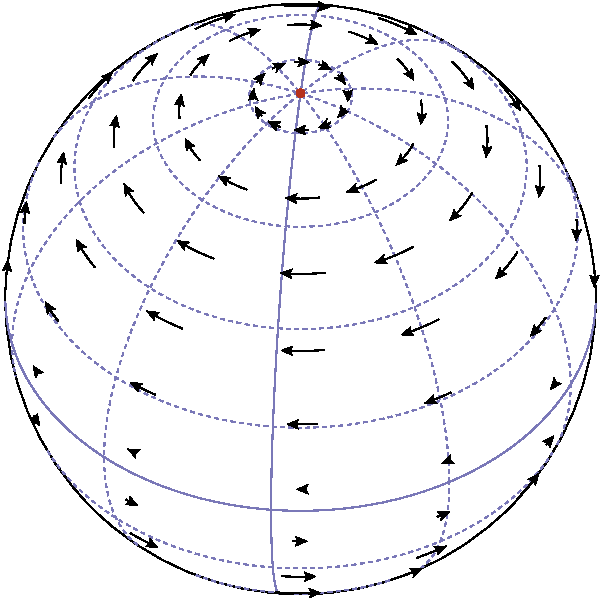
\includegraphics[scale=0.7]{images/Xlm1m0.pdf}
\subcaption{Re $X_{1 0}(\theta,\varphi)$}\label{fig:basis_xlmzlm_a}
\end{minipage}%
\begin{minipage}[b]{.5\linewidth}
\centering
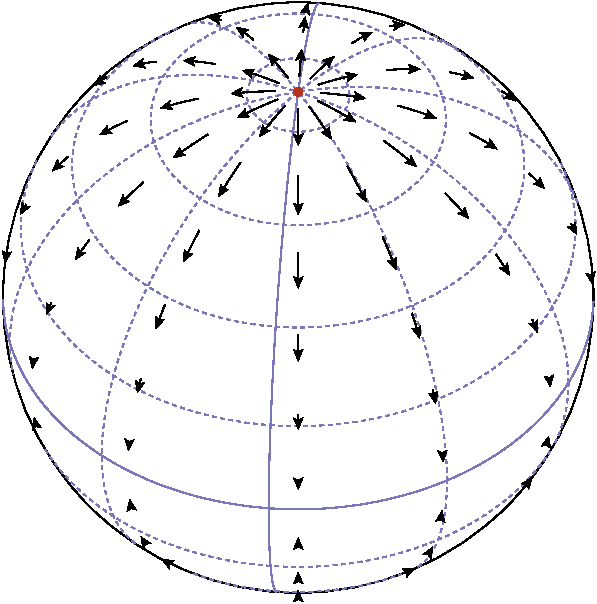
\includegraphics[scale=0.7]{images/Zlm1m0.pdf}
\subcaption{Re $Z_{1 0}(\theta,\varphi)$}\label{fig:basis_xlmzlm_b}
\end{minipage}

\ \\

\begin{minipage}[b]{.5\linewidth}
\centering
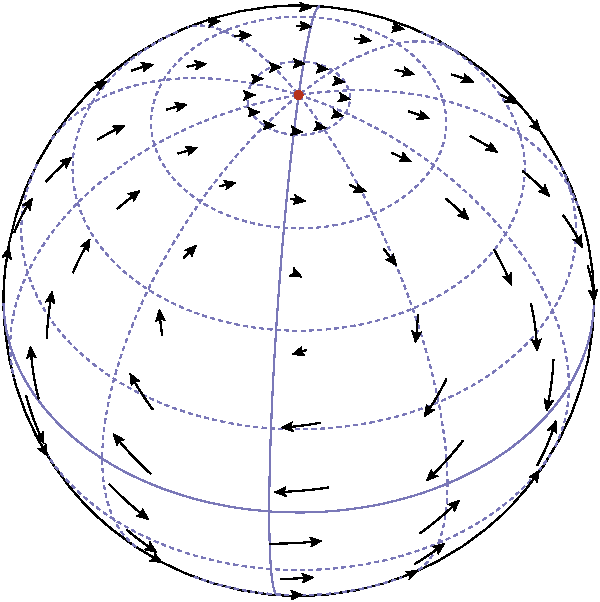
\includegraphics[scale=0.7]{images/Xlm2m1.pdf}
\subcaption{Re $X_{2 1}(\theta,\varphi)$}\label{fig:basis_xlmzlm_c}
\end{minipage}%
\begin{minipage}[b]{.5\linewidth}
\centering
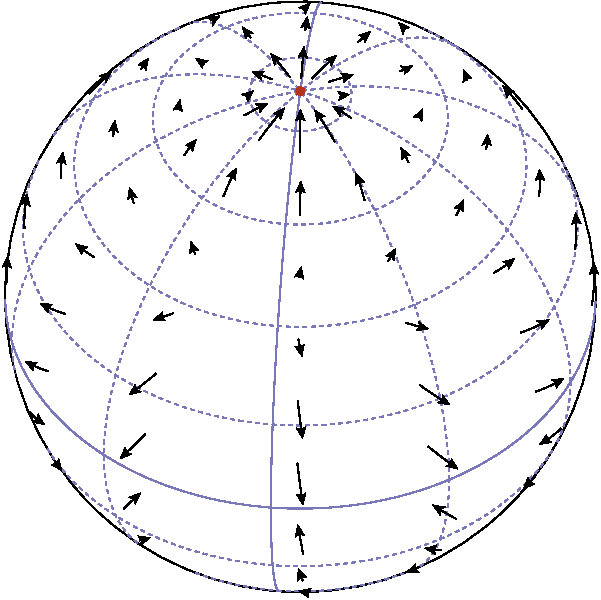
\includegraphics[scale=0.7]{images/Zlm2m1.pdf}
\subcaption{Re $Z_{2 1}(\theta,\varphi)$}\label{fig:basis_xlmzlm_d}
\end{minipage}

\caption{Real part of $X_{\ell m}$ and $Z_{\ell m}$ for $\ell=1, m=0$ and
$\ell=2, m=1$. The red point corresponds to the north pole, the solid lines to
equator, meridian and anti-meridian. For $m=0$ the vector spherical harmonics
$X_{\ell m}$ and $Z_{\ell m}$ are real and independent of $\varphi$.}
\label{fig:basis_xlmzlm}
\end{figure}

The multipole basis is well adapted to the isotropy of space:
The basis functions of the multipole basis are eigenfunctions to $\hat E$,
$\hat{\vec{J}}^2$, $\hat{J}_z$ und $\hat P$:
\begin{align}
\hat{E} \ket{\omega,\ell,m,P} &= \hbar\omega \ket{\omega,\ell,m,P} \\
\hat{\vec J}^2 \ket{\omega,\ell,m,P} &= \hbar^2 \ell(\ell+1) \ket{\omega,\ell,m,P} \\
\hat{J}_z \ket{\omega,\ell,m,P} &= \hbar m \ket{\omega,\ell,m,P} \\
\hat{P} \ket{\omega,\ell,m,P} &= \pm \ket{\omega,\ell,m,P}
\end{align}
Using the multipole basis source-free solutions of the Helmholtz equation can be expanded by
\begin{equation}
\vec E(\vec K) = \sum_{P=\PE,\PM} \sum_{\ell=1}^\infty \sum_{m=-\ell}^\ell \alpha_{\ell,m,P} \braket{\vec K \, | \, \omega, \ell, m, P}.
\end{equation}


\section{Matrix elements for the change of basis}

The matrix elements for the change of basis from plane wave basis to multipole
basis can be calculated using their representations in $k$-space. For the
change of a $\TE$-polarized plane wave to an electric multipole wave we obtain
\begin{align}
\nonumber
&\braket{\vec{k},\omega,\pm,\TE \, |\, \omega^\prime,\ell,m,\PE} = \int \mathrm{d}^3\vec K^\prime \, \braket{\vec{k},\omega,\pm,\TE \, |\, \vec{K}^\prime} \braket{\vec{K}^\prime \, | \, \omega^\prime,\ell,m,\PE} \\
\label{eq:3_TEE}
&\sep = \int \mathrm{d}^3\vec K^\prime \, \frac{\c}{\omega^\prime} \sqrt{\left| \frac{\omega}{\c k_z} \right|} \, \delta\left(\vec k^\prime - \vec k\right) \, \delta\left(K_z^\prime \mp k_z\right) \delta\left(K^\prime-\frac{\omega^\prime}{\c}\right) \, \frac{\partial_\varphi \Ylm{\ell m}\left(\theta^\prime,\varphi^\prime\right)}{\sin\theta^\prime \sqrt{\ell(\ell+1)}}.
\end{align}
Changing to spherical coordinates the product of delta functions becomes
\begin{equation}
\label{eq:_TEE_zwischenschritt}
\delta\left(\vec k^\prime - \vec k\right) \, \delta\left(K_z^\prime \mp k_z\right) \, \delta\left(K^\prime-\frac{\omega^\prime}{\c}\right) =
\frac{\delta\left(\theta^\prime-\theta^\pm\right) \, \delta\left(\varphi^\prime-\varphi\right) \, \delta\left(K^\prime-\frac{\omega}{\c}\right)}{\frac{\omega^2}{\c^2} \sin\theta^\pm} \, \delta\left(K^\prime-\frac{\omega^\prime}{\c}\right)
\end{equation}
and the integration variables are now $K^\prime$, $\theta^\prime$, and $\varphi^\prime$.
Inserting \eqref{eq:_TEE_zwischenschritt} into \eqref{eq:3_TEE} yields
\begin{align}
&\braket{\vec{k},\omega,\pm,\TE \, |\, \omega^\prime,\ell,m,\PE} = \int \mathrm{d}K^\prime \mathrm{d}\theta^\prime \mathrm{d}\varphi^\prime {K^\prime}^2 \sin\theta^\prime \frac{\c}{\omega^\prime} \sqrt{\left| \frac{\omega}{\c k_z} \right|} \\
&\sep\sep\sep\sep\times \frac{\delta\left(\theta^\prime-\theta^\pm\right) \, \delta\left(\varphi^\prime-\varphi\right) \, \delta\left(K^\prime-\frac{\omega}{\c}\right)}{\frac{\omega^2}{\c^2} \sin\theta^\pm} \, \delta\left(K^\prime-\frac{\omega^\prime}{\c}\right) \frac{\partial_\varphi \Ylm{\ell m}\left(\theta^\prime,\varphi^\prime\right)}{\sin\theta^\prime \sqrt{\ell(\ell+1)}}.
\end{align}
The integration of the angular part changes $\theta^\prime\to\theta^\pm$ and 
$\varphi^\prime\to\varphi$, the integration of the radial part yields the delta function
$\delta\left(\omega/\c-\omega^\prime/\c\right)$. After cancelling we arrive at
\begin{equation}
\braket{\vec{k},\omega,\pm,\TE \, |\, \omega^\prime,\ell,m,\PE} 
= \frac{\c}{\omega^\prime} \sqrt{\left|\frac{\omega}{\c k_z}\right|} \, \delta\left(\frac{\omega^\prime}{\c}-\frac{\omega}{\c}\right) \, \frac{\partial_\varphi \Ylm{\ell m}\left(\theta^\pm,\varphi\right)}{\sin\theta^\pm \sqrt{\ell(\ell+1)}}.
\end{equation}
The derivative with respect to $\varphi$ brings up a factor $\imag m$ and
after exploiting the identity \eqref{eq:notation_cossintheta} $k = \omega/\c \sin\theta^\pm$ we finally
obtain
\begin{equation}
\label{eq:basis_change_1}
\braket{\vec{k},\omega,\pm,\TE \, |\, \omega^\prime,\ell,m,\PE} 
= \frac{\imag m}{k} \sqrt{\left|\frac{\omega}{\c k_z}\right|} \, \delta\left(\frac{\omega}{\c}-\frac{\omega^\prime}{\c}\right) \, \frac{\Ylm{\ell m}(\theta^\pm,\varphi)}{\sqrt{\ell(\ell+1)}}.
\end{equation}
For the change from a $\TE$ polarized plane wave to an electric multipole wave
one finds
\begin{equation}
\label{eq:basis_change_2}
\braket{\vec{k},\omega,\pm,\TE \, | \, \omega^\prime,\ell,m,\PM}
= \frac{\c}{\omega} \sqrt{\left| \frac{\omega}{\c k_z} \right|} \, \delta\left(\frac{\omega}{\c}-\frac{\omega^\prime}{\c}\right) \, \frac{\partial_\theta \Ylm{\ell m}(\theta^\pm,\varphi)}{\sqrt{\ell(\ell+1)}}.
\end{equation}
The two remaining matrix elements are given by
\begin{align}
\label{eq:basis_change_3}
\braket{\vec{k},\omega,\pm,\TM \, | \, \omega^\prime, \ell, m, M} &= -\braket{\vec{k},\omega,\pm,\TE \, | \, \omega^\prime, \ell, m, E}, \\
\label{eq:basis_change_4}
\braket{\vec{k},\omega,\pm,\TM \, | \, \omega^\prime, \ell, m, E} &= \braket{\vec{k},\omega,\pm,\TE \, | \, \omega^\prime, \ell, m, M}.
\end{align}

The plane wave basis is well adapted for propagation and reflection at a plane,
the multipole basis is well adapted for reflection at a sphere. Before we apply
the scattering formula to the plane--sphere geometry in chapter
\ref{chapter_scattering_ps}, we study reflection properties of electromagnetic
waves at planes and spheres in the next chapter, and apply the scattering
formula to the plane--plane geometry in chapter \ref{chapter_scattering_pp}.
